% Options for packages loaded elsewhere
\PassOptionsToPackage{unicode}{hyperref}
\PassOptionsToPackage{hyphens}{url}
%
\documentclass[
]{article}
\usepackage{amsmath,amssymb}
\usepackage{iftex}
\ifPDFTeX
  \usepackage[T1]{fontenc}
  \usepackage[utf8]{inputenc}
  \usepackage{textcomp} % provide euro and other symbols
\else % if luatex or xetex
  \usepackage{unicode-math} % this also loads fontspec
  \defaultfontfeatures{Scale=MatchLowercase}
  \defaultfontfeatures[\rmfamily]{Ligatures=TeX,Scale=1}
\fi
\usepackage{lmodern}
\ifPDFTeX\else
  % xetex/luatex font selection
\fi
% Use upquote if available, for straight quotes in verbatim environments
\IfFileExists{upquote.sty}{\usepackage{upquote}}{}
\IfFileExists{microtype.sty}{% use microtype if available
  \usepackage[]{microtype}
  \UseMicrotypeSet[protrusion]{basicmath} % disable protrusion for tt fonts
}{}
\makeatletter
\@ifundefined{KOMAClassName}{% if non-KOMA class
  \IfFileExists{parskip.sty}{%
    \usepackage{parskip}
  }{% else
    \setlength{\parindent}{0pt}
    \setlength{\parskip}{6pt plus 2pt minus 1pt}}
}{% if KOMA class
  \KOMAoptions{parskip=half}}
\makeatother
\usepackage{xcolor}
\usepackage[margin=1in]{geometry}
\usepackage{longtable,booktabs,array}
\usepackage{calc} % for calculating minipage widths
% Correct order of tables after \paragraph or \subparagraph
\usepackage{etoolbox}
\makeatletter
\patchcmd\longtable{\par}{\if@noskipsec\mbox{}\fi\par}{}{}
\makeatother
% Allow footnotes in longtable head/foot
\IfFileExists{footnotehyper.sty}{\usepackage{footnotehyper}}{\usepackage{footnote}}
\makesavenoteenv{longtable}
\usepackage{graphicx}
\makeatletter
\newsavebox\pandoc@box
\newcommand*\pandocbounded[1]{% scales image to fit in text height/width
  \sbox\pandoc@box{#1}%
  \Gscale@div\@tempa{\textheight}{\dimexpr\ht\pandoc@box+\dp\pandoc@box\relax}%
  \Gscale@div\@tempb{\linewidth}{\wd\pandoc@box}%
  \ifdim\@tempb\p@<\@tempa\p@\let\@tempa\@tempb\fi% select the smaller of both
  \ifdim\@tempa\p@<\p@\scalebox{\@tempa}{\usebox\pandoc@box}%
  \else\usebox{\pandoc@box}%
  \fi%
}
% Set default figure placement to htbp
\def\fps@figure{htbp}
\makeatother
\setlength{\emergencystretch}{3em} % prevent overfull lines
\providecommand{\tightlist}{%
  \setlength{\itemsep}{0pt}\setlength{\parskip}{0pt}}
\setcounter{secnumdepth}{-\maxdimen} % remove section numbering
\usepackage{booktabs}
\usepackage{threeparttable}
\usepackage[utf8]{inputenc}
\usepackage[T1]{fontenc}
\usepackage{amsmath}
\usepackage{tabularx}
\usepackage{threeparttable}
\usepackage{pdflscape}
\usepackage{float}
\floatplacement{figure}{H}
\usepackage{subcaption}
\usepackage{booktabs}
\usepackage{longtable}
\usepackage{array}
\usepackage{multirow}
\usepackage{wrapfig}
\usepackage{float}
\usepackage{colortbl}
\usepackage{pdflscape}
\usepackage{tabu}
\usepackage{threeparttable}
\usepackage{threeparttablex}
\usepackage[normalem]{ulem}
\usepackage{makecell}
\usepackage{xcolor}
\usepackage[]{natbib}
\bibliographystyle{apalike}
\usepackage{bookmark}
\IfFileExists{xurl.sty}{\usepackage{xurl}}{} % add URL line breaks if available
\urlstyle{same}
\hypersetup{
  pdftitle={Imagine -- An Exploratory Analysis},
  hidelinks,
  pdfcreator={LaTeX via pandoc}}

\title{Imagine -- An Exploratory Analysis}
\author{}
\date{\vspace{-2.5em}2026-03-10}

\begin{document}
\maketitle

\subsubsection{Before we start}\label{before-we-start}

The data used in this report is the same you used for your analysis. I
used the mean ratings for each dimension (factivity, intentionality,
pictoriality) and scaled them. In the upcoming weeks, I will also adapt
the scripts as to use the ratings of both coders to account for
between-coder variance. I just didn't have the time to do everything.
Since manual sense annotations are not yet available, I wrote the
pipeline based on a clustering of the the data on the three provided
annotation dimensions. We can later just replace them with the actual
annotations.

\subsubsection{Pre-analysis}\label{pre-analysis}

Table \ref{tab:pairwisePearsonDimensions}.

\begin{table}[H]
\centering
\caption{\label{tab:pairwisePearsonDimensions}Pairwise Pearson Correlation}
\centering
\begin{tabular}[t]{lrrr}
\toprule
  & intentionality & factivity & pictoriality\\
\midrule
intentionality & 1 & -0.242 & 0.374\\
factivity &  & 1.000 & -0.222\\
pictoriality &  &  & 1.000\\
\bottomrule
\end{tabular}
\end{table}

Figure \ref{fig:gmmBIC}

\begin{figure}
\centering
\pandocbounded{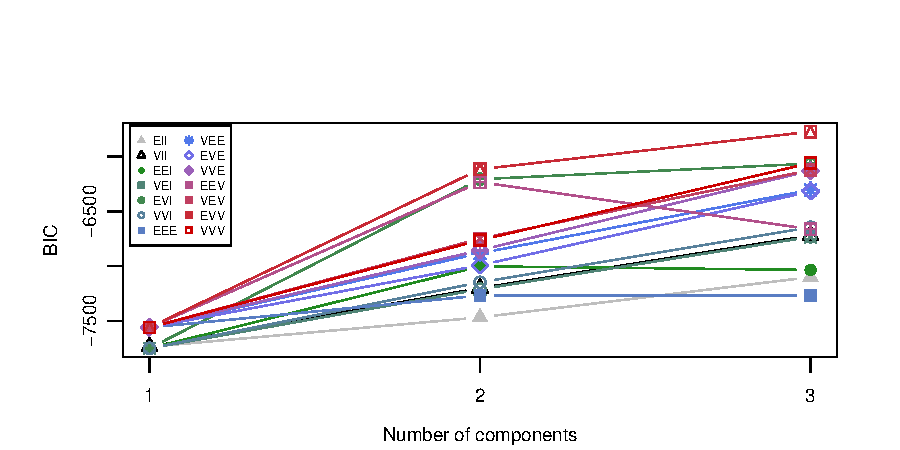
\includegraphics[keepaspectratio]{imagine_report_files/figure-latex/unnamed-chunk-4-1.pdf}}
\caption{BIC for Gaussian mixture models.\label{fig:gmmBIC}}
\end{figure}

Figure \ref{fig:pcaGMM}.

\begin{figure}
\centering
\pandocbounded{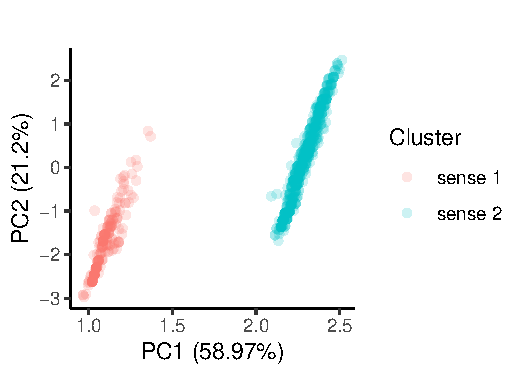
\includegraphics[keepaspectratio]{imagine_report_files/figure-latex/unnamed-chunk-5-1.pdf}}
\caption{PCA of annotation space with latent sense
clusters.\label{fig:pcaGMM}}
\end{figure}

\begin{figure}

{\centering 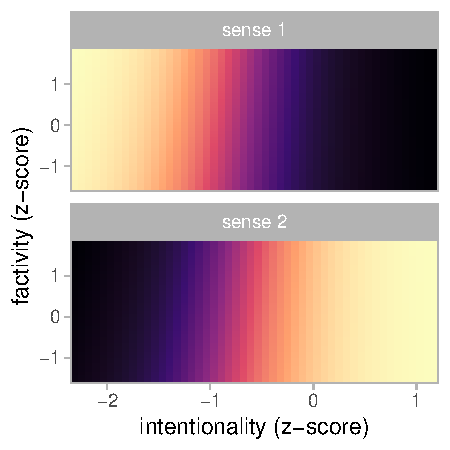
\includegraphics[width=.32\linewidth]{imagine_report_files/figure-latex/unnamed-chunk-6-1} 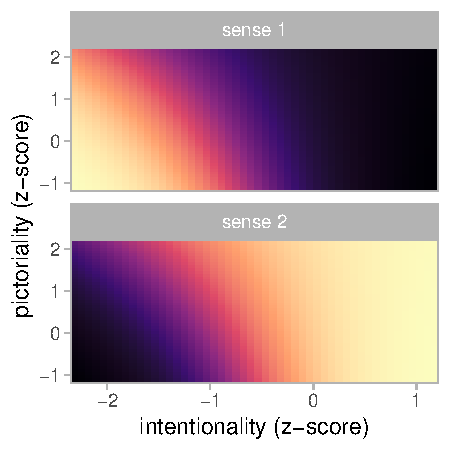
\includegraphics[width=.32\linewidth]{imagine_report_files/figure-latex/unnamed-chunk-6-2} 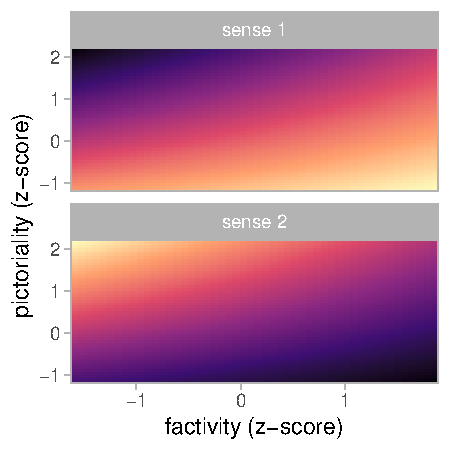
\includegraphics[width=.32\linewidth]{imagine_report_files/figure-latex/unnamed-chunk-6-3} 

}

\caption{Predicted sense probability based on GLM with ridge regularization for 2-way interactions. The third dimension is held constant at the median value.The lighter the color, the higher the probability.\label{fig:xEffects}}\label{fig:unnamed-chunk-6}
\end{figure}

\begin{figure}
\centering
\pandocbounded{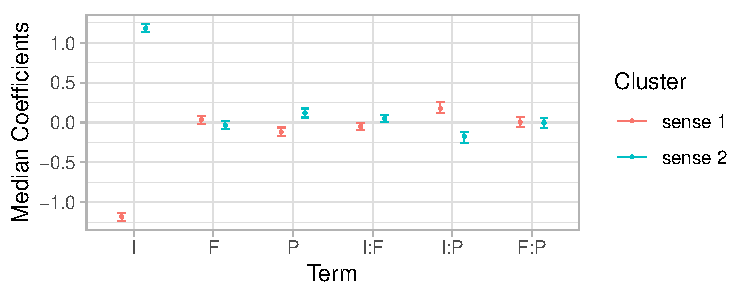
\includegraphics[keepaspectratio]{imagine_report_files/figure-latex/unnamed-chunk-7-1.pdf}}
\caption{Bootstrapped Coefficients (n = 500) with 95\%
CI.\label{fig:bootstrapping}}
\end{figure}

\section{Embedding analysis}\label{embedding-analysis}

\subsection{Centroids}\label{centroids}

\begin{figure}
    \centering
    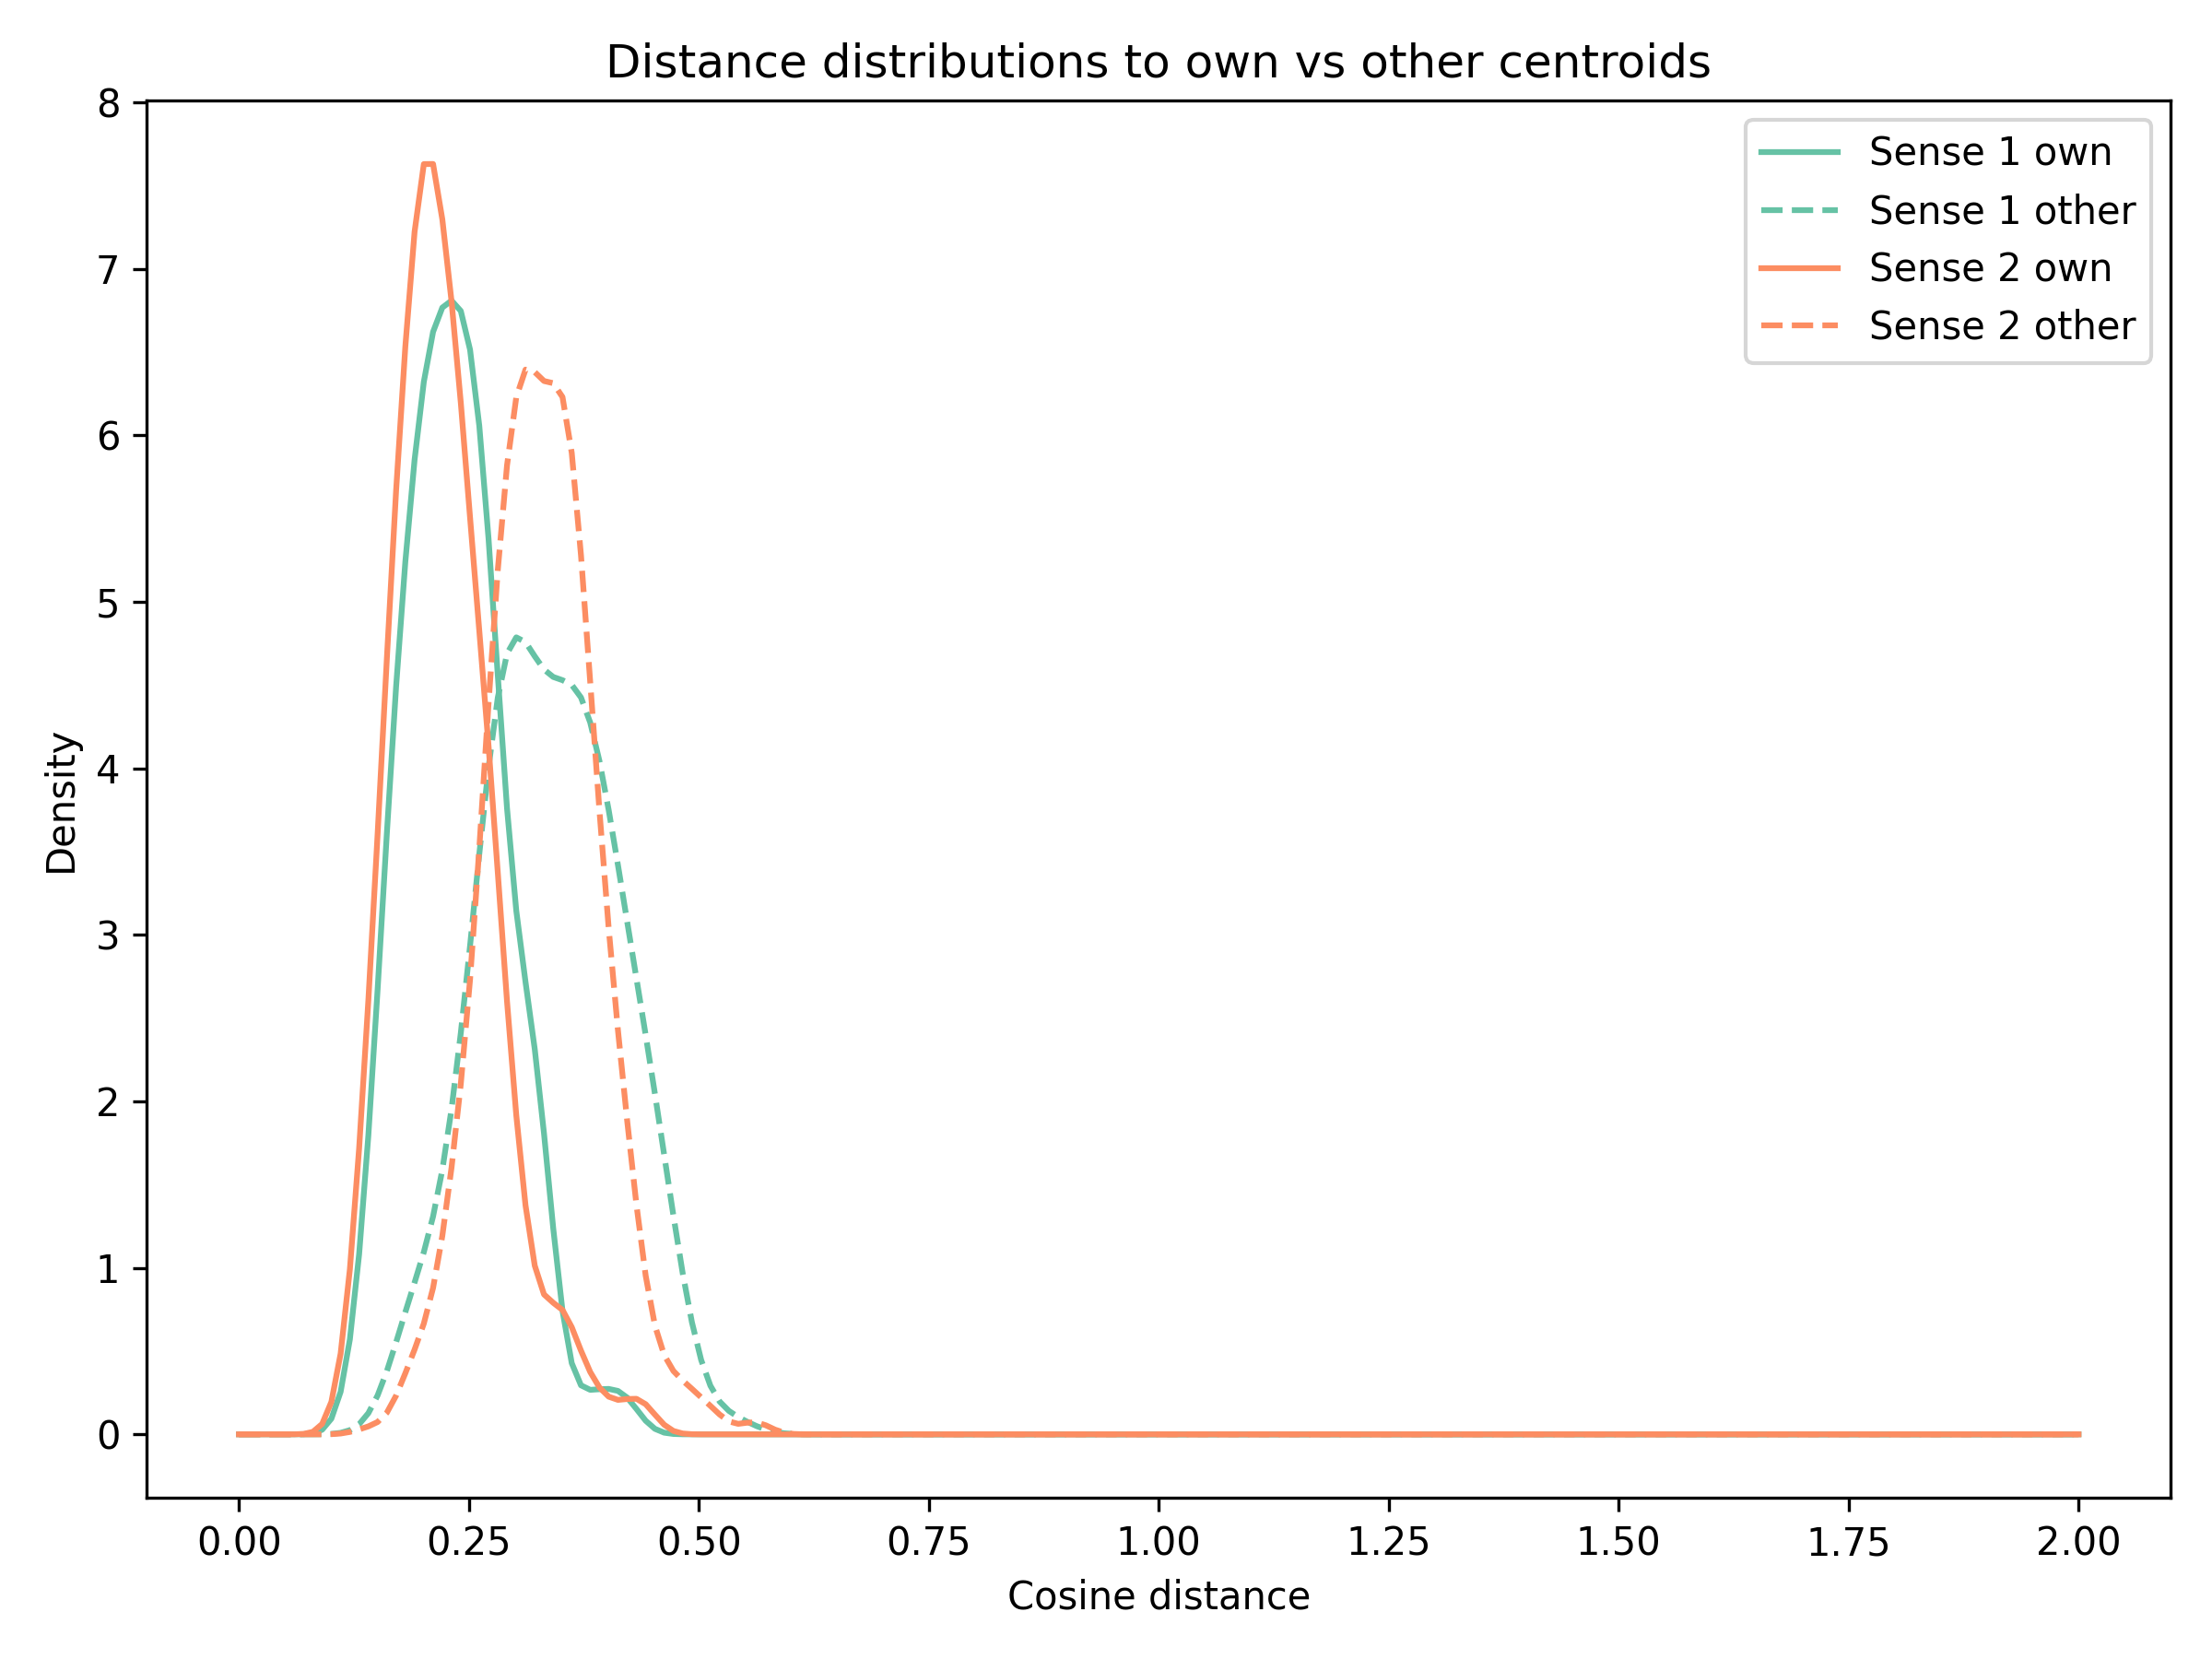
\includegraphics[width=0.5\linewidth]{../../output/plots/overlap_density.png}
    \caption{Caption}
    \label{fig:placeholder}
\end{figure}

\begin{figure}
\centering
    \begin{subfigure}[b]{0.6\textwidth}
    \centering
    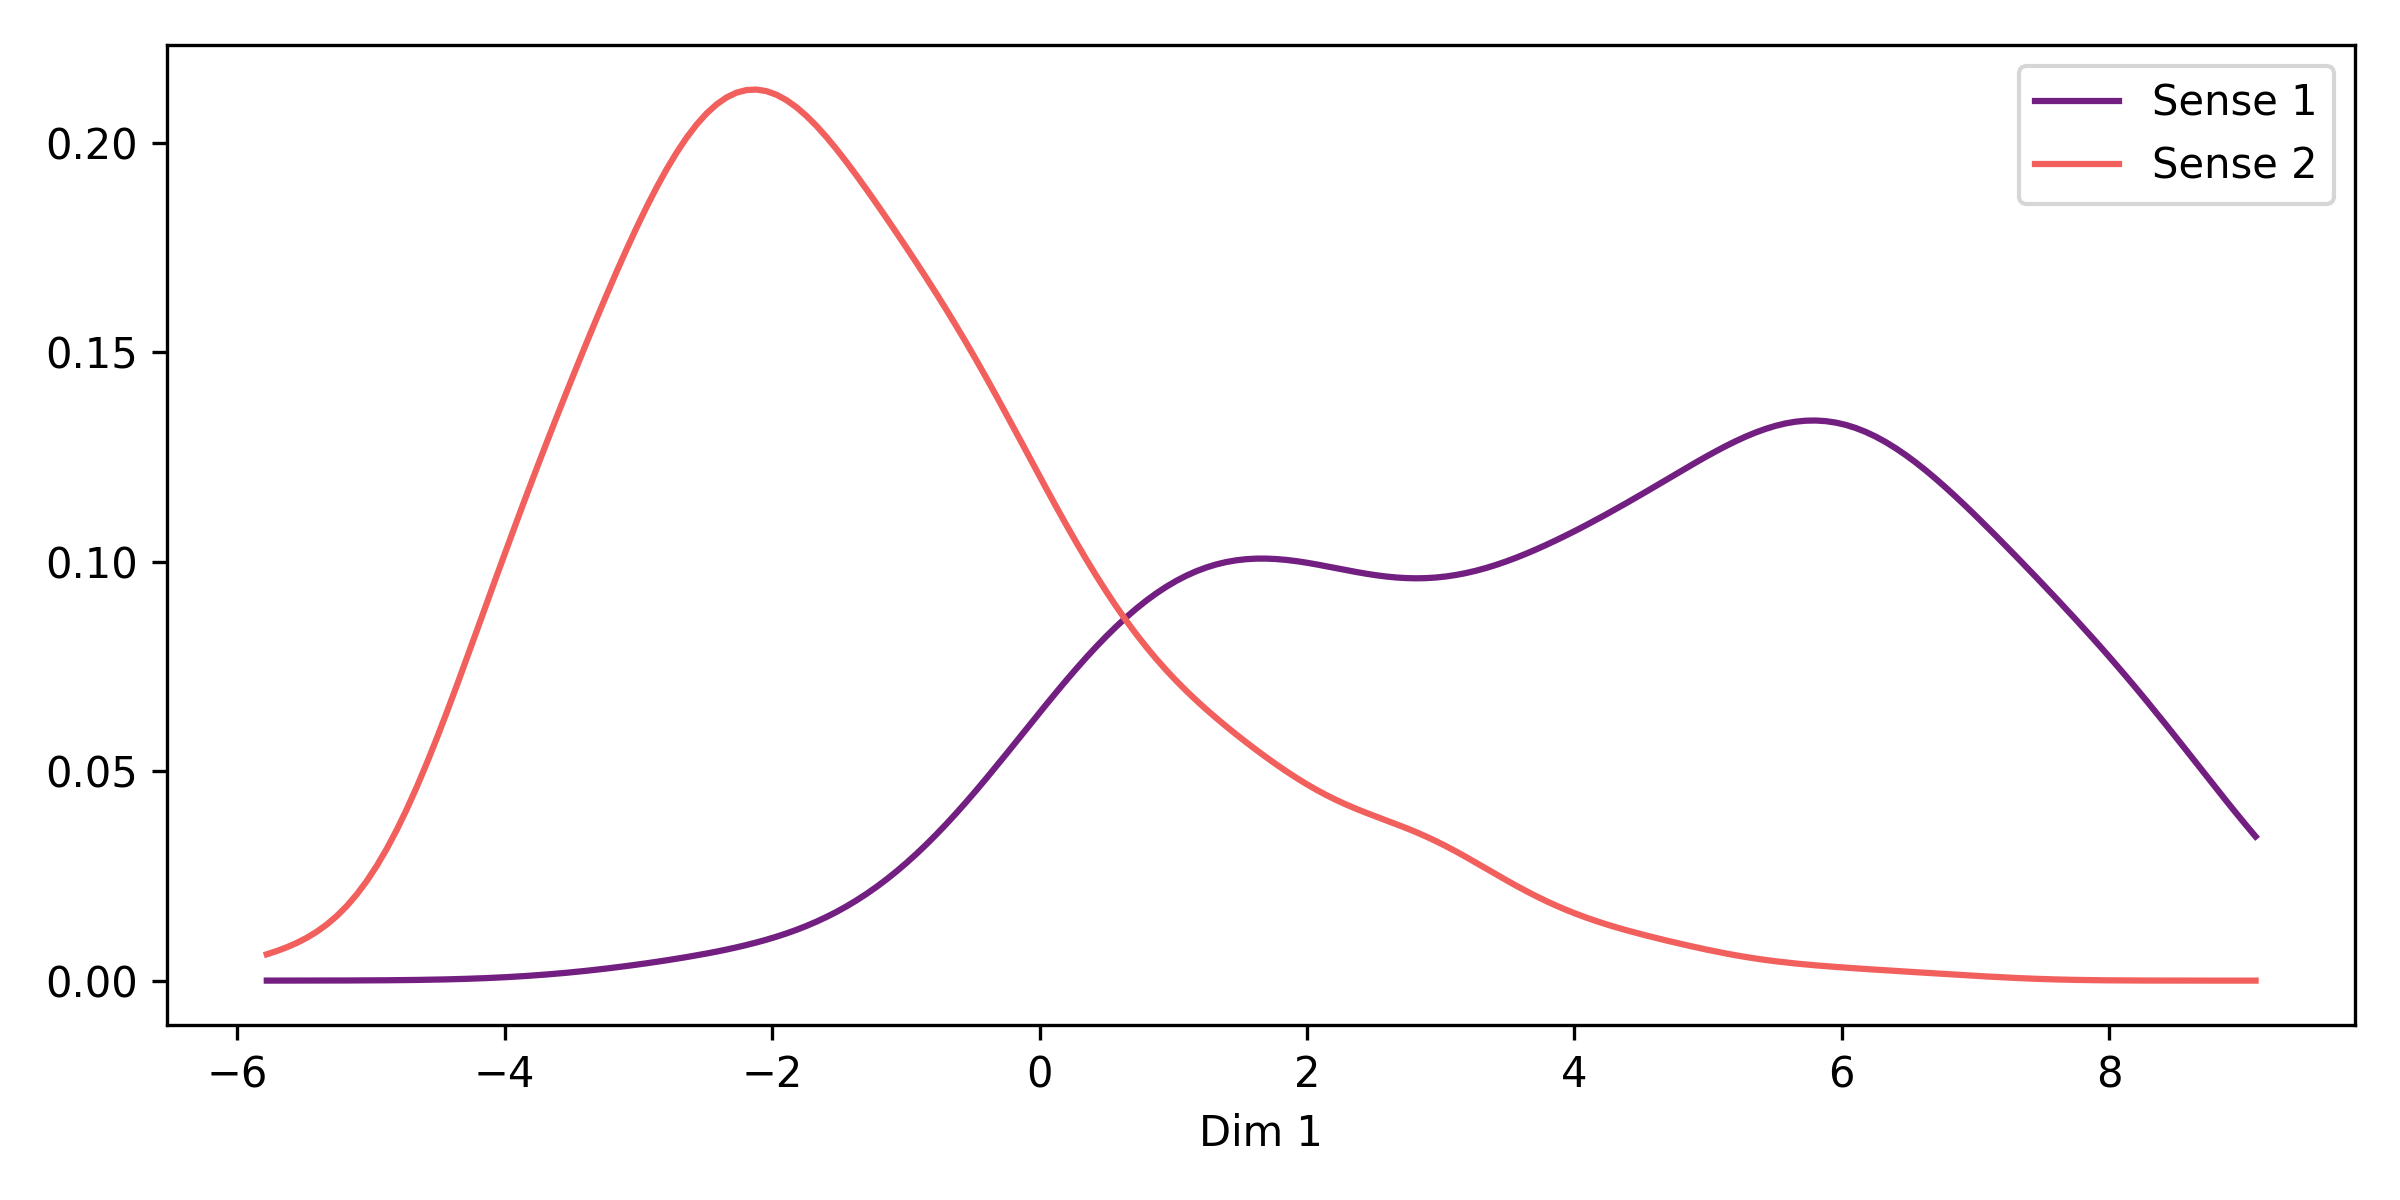
\includegraphics[width=\textwidth]{../../output/plots/kde1D_embeddings.png}
    \caption{\label{fig:image1}}
    \end{subfigure}
    \hfill
    \begin{subfigure}[b]{0.38\textwidth}
    \centering
    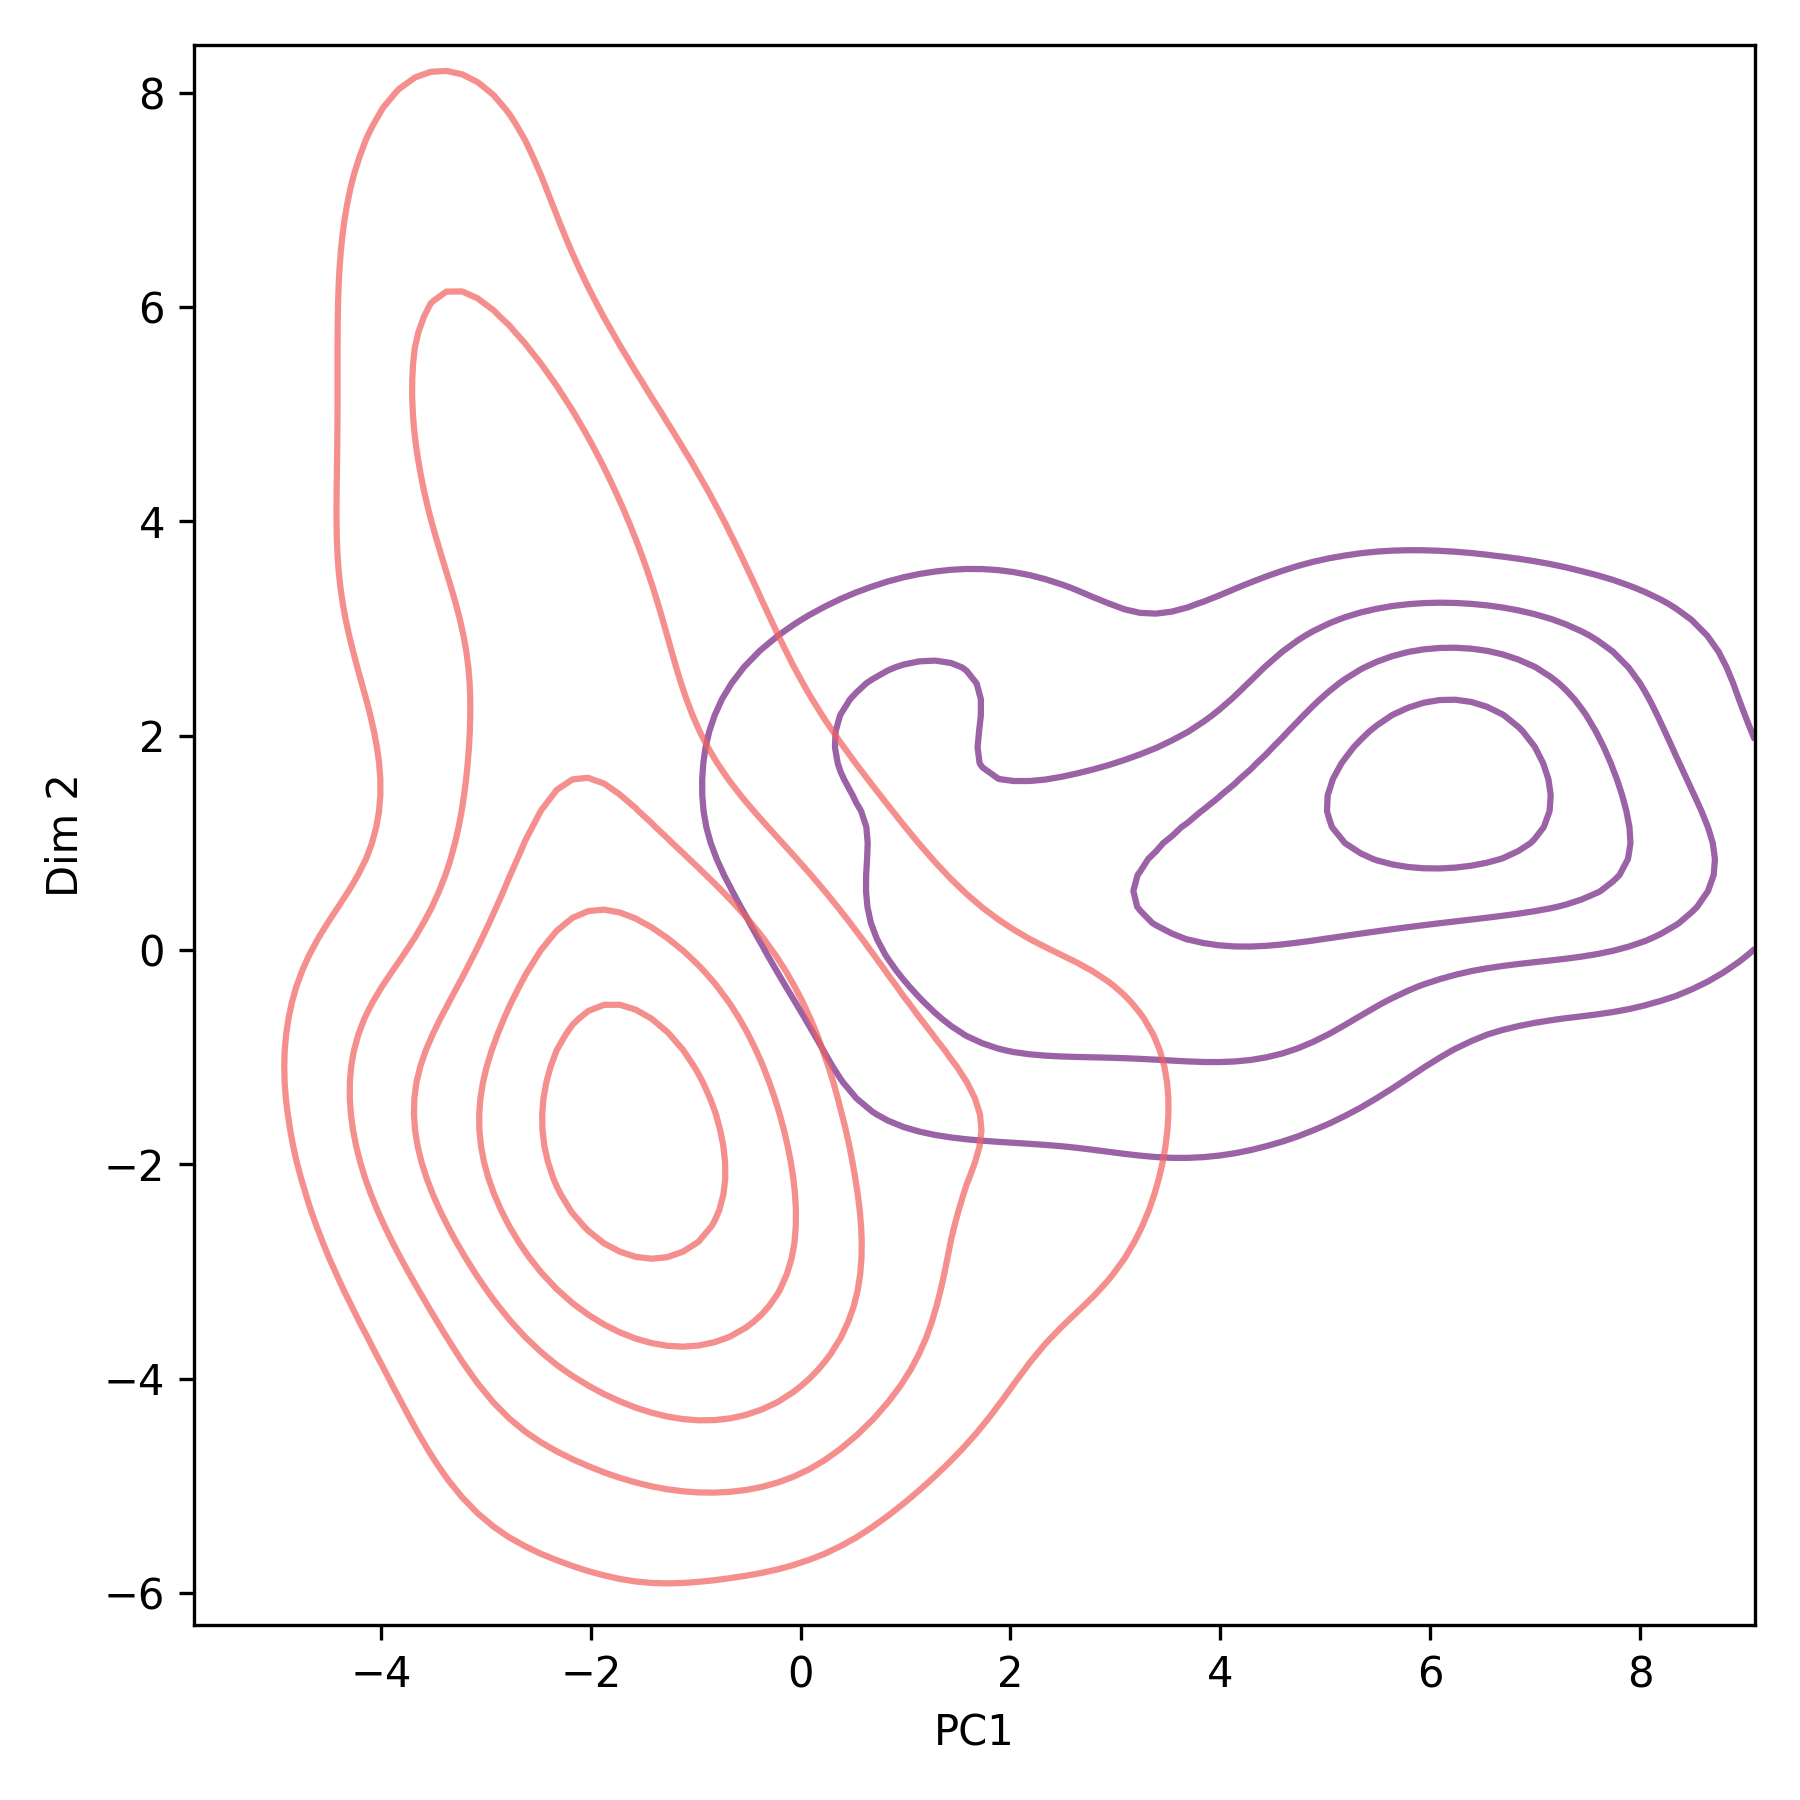
\includegraphics[width=0.9\textwidth]{../../output/plots/kde2D_embeddings.png}
    \caption{\label{fig:image2}}
    \end{subfigure}
\end{figure}

\subsection{Embedding similarity vs sense
similarity}\label{embedding-similarity-vs-sense-similarity}

\begin{figure}
    \centering
    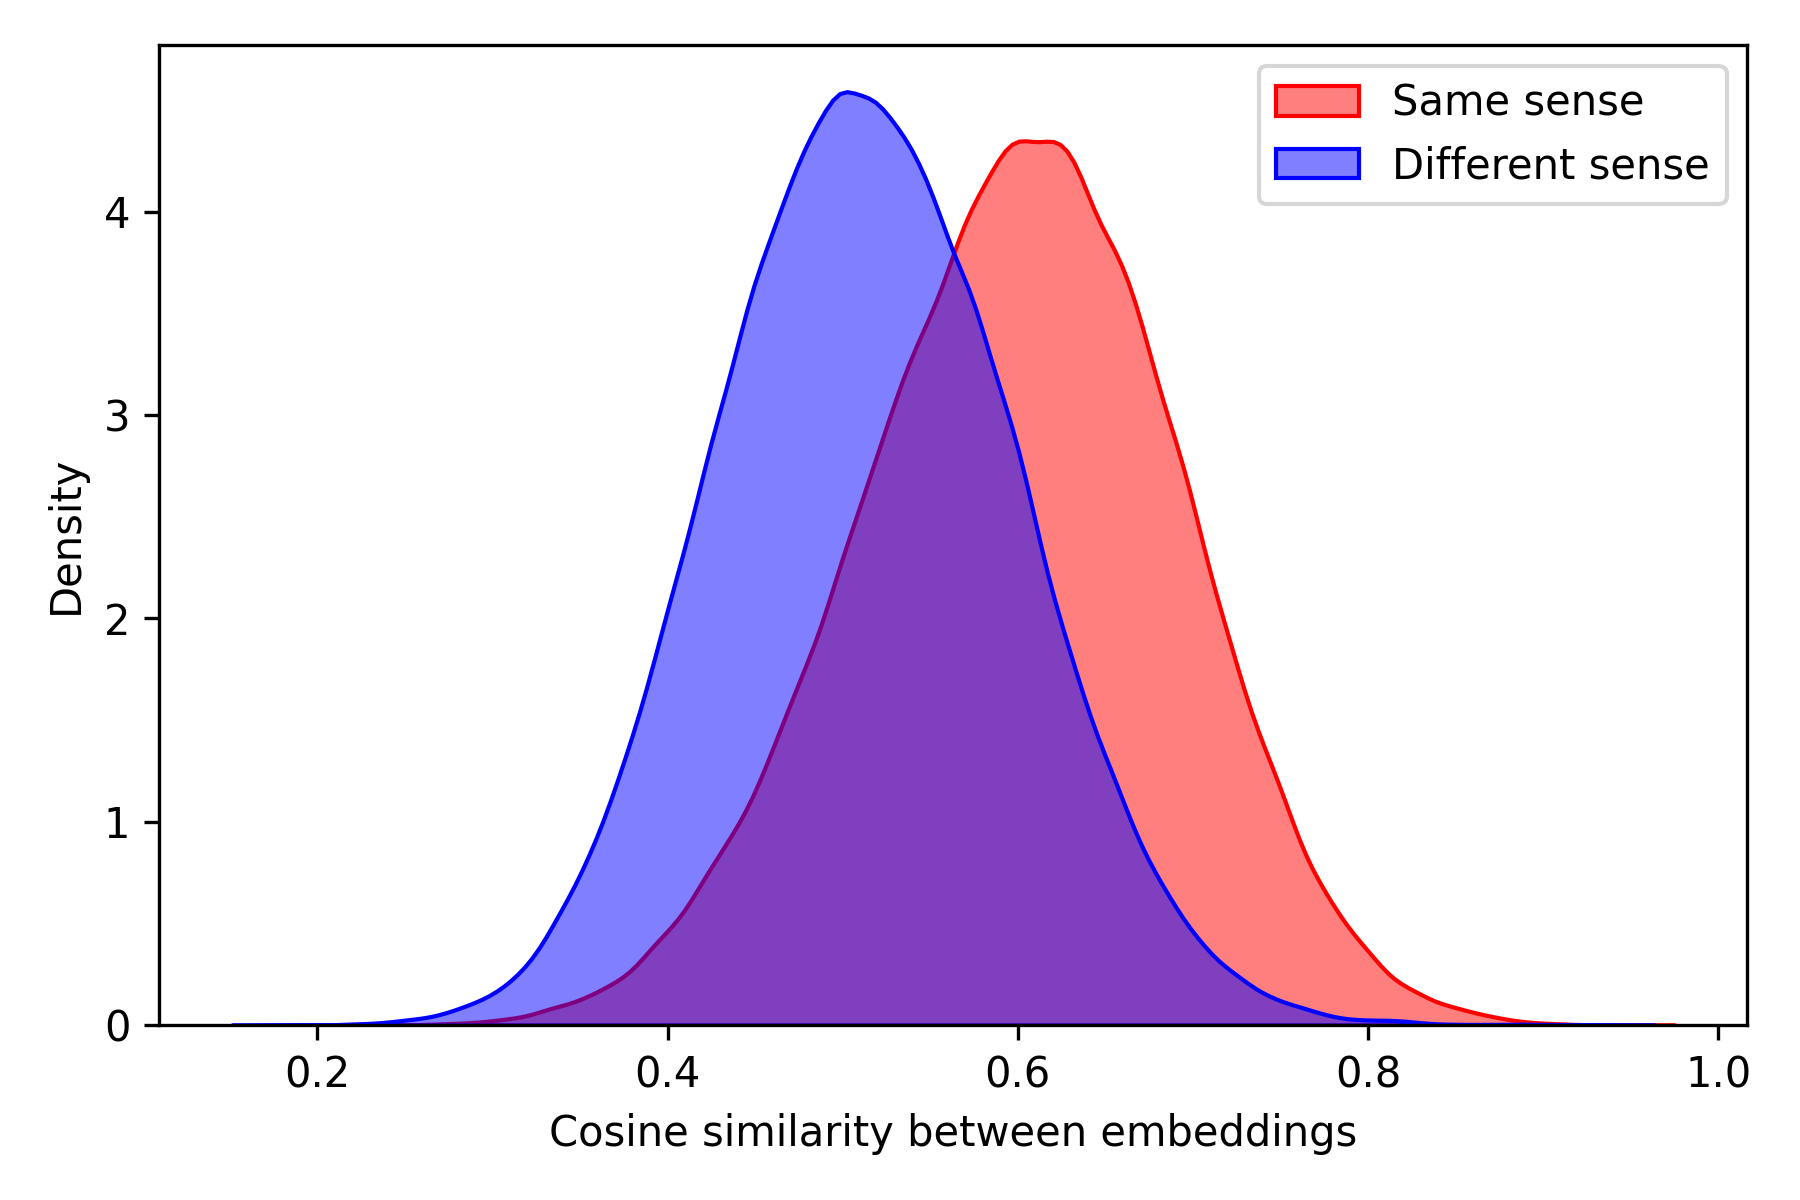
\includegraphics[width=0.5\linewidth]{../../output/plots/embedding_vs_sense_similarity.png}
    \caption{Caption}
    \label{fig:placeholder}
\end{figure}

\subsection{Senses under embedding
projection}\label{senses-under-embedding-projection}

To examine how sentence embeddings capture the three annotated semantic
dimensions (\emph{intentionality}, \emph{factivity}, and
\emph{pictoriality}), we trained simple linear regression models
predicting each z-scaled dimension from the sentence embeddings. The
regression coefficients define a direction in embedding space along
which the dimension increases. By projecting each sentence embedding
onto these directions, we obtain an embedding-based estimate for that
dimension. This procedure was repeated for all three dimensions,
resulting in a 3D projection of each sentence in the space spanned by
the semantic dimensions.

Let \(\mathbf{X} \in \mathbb{R}^{n \times d}\) denote the matrix of
sentence embeddings, where \(n\) is the number of sentences and \(d\)
the embedding dimension. Let \(\mathbf{y}^{(k)} \in \mathbb{R}^n\) be
the vector of z-scaled ratings for semantic dimension
\(k \in \{\text{intentionality, factivity, pictoriality}\}\).

We fit a simple linear regression model for each dimension:

\[
\mathbf{y}^{(k)} = \mathbf{X} \boldsymbol{\beta}^{(k)} + \boldsymbol{\epsilon}^{(k)},
\]

where \(\boldsymbol{\beta}^{(k)} \in \mathbb{R}^d\) is the vector of
regression coefficients and \(\boldsymbol{\epsilon}^{(k)}\) is the
residual vector. The estimated coefficients
\(\hat{\boldsymbol{\beta}}^{(k)}\) define a direction in embedding space
corresponding to increases in dimension \(k\).

The projection of each sentence embedding \(\mathbf{x}_i\) onto this
direction provides an embedding-based estimate of the semantic
dimension:

\[
\hat{y}^{(k)}_i = \mathbf{x}_i^\top \hat{\boldsymbol{\beta}}^{(k)}, \quad i = 1, \dots, n.
\]

By computing these projections for all three dimensions, each sentence
is represented in a 3D space spanned by the semantic directions,
allowing visualization and analysis of how embeddings capture the
annotated semantic structure.

Figure \ref{fig:3Dprojection} shows 3D projection of sentence embeddings
onto the directions corresponding to the annotated semantic dimensions
(intentionality, factivity, and pictoriality). It reveals that the sense
clusters are well-separated in this space. This indicates that the
latent embedding space encodes information aligned with the annotated
dimensions. In other words, the directions learned via linear regression
effectively capture the semantic structure underlying the sense
distinctions. The clear separation suggests that even a simple linear
mapping from embeddings to semantic dimensions is sufficient to
discriminate the senses, highlighting that the embeddings intrinsically
encode patterns that correspond to the interpretive distinctions
annotated in the dataset.

\begin{figure}
    \centering
    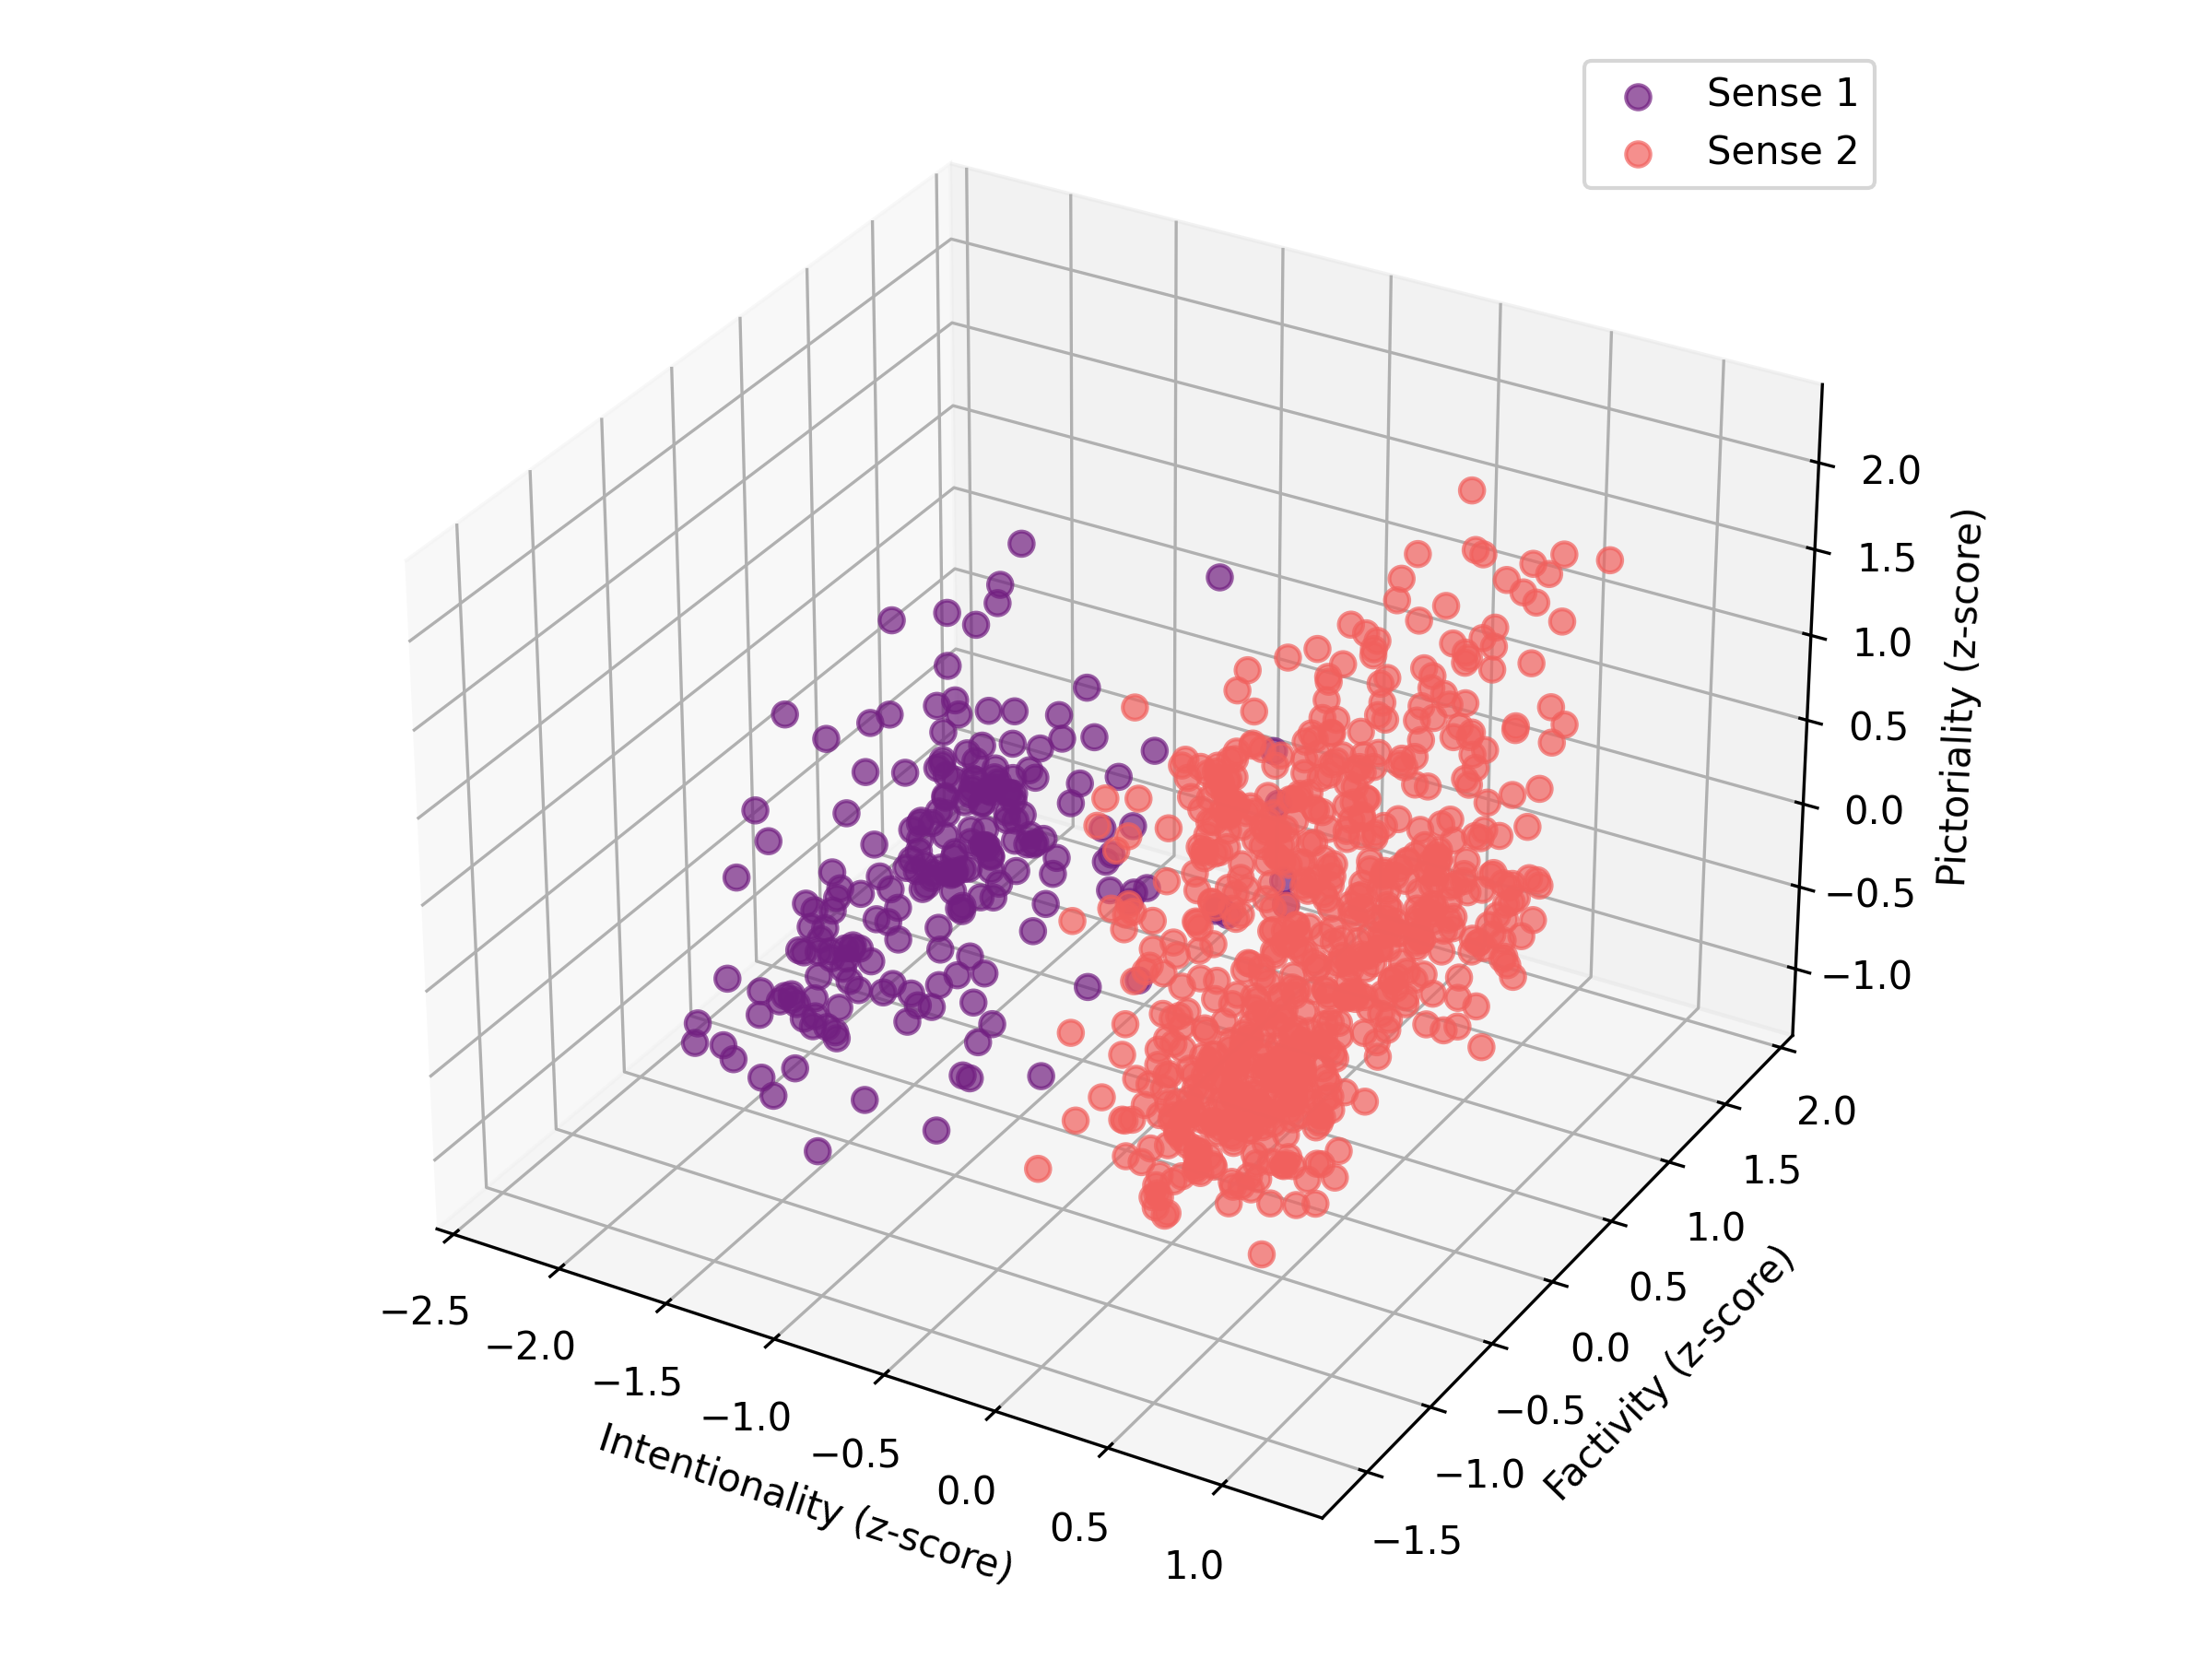
\includegraphics[width=0.5\linewidth]{../../output/plots/embedding_projection_3D.png}
    \caption{3D embedding projections. Dimensions have been rescaled to $z$-scores.}
    \label{fig:3Dprojection}
\end{figure}

Figure \ref{fig:2Dprojection} depicts 2-dimensional for all combinations
of dimensions. For projections for factivity and intentionality (Fig.
\ref{fig:2D_IF}), sense 1 was predominantly associated with high
factivity and low intentionality, whereas sense 2 showed the opposite
pattern. Both distributions exhibited slight bimodality. In the
pictoriality--intentionality projection (Fig. \ref{fig:2D_IP}),
pictoriality contributed minimally, with sense clusters largely
segregated along the intentionality axis. In contrast, the
pictoriality--factivity projection (Fig. \ref{fig:2D_FP}) revealed
substantial overlap between the two senses, indicating that the senses
are not well distinguished along this dimension pair. These results
suggest that the distinctions between the senses are primarily encoded
along the intentionality and factivity dimensions, whereas pictoriality
alone does not reliably differentiate sense membership.

\begin{figure}
\centering
    \caption{2D embedding projections. Dimensions have been rescaled to $z$-scores.}
    \label{fig:2Dprojection}
    \begin{subfigure}[b]{0.30\textwidth}
    \centering
    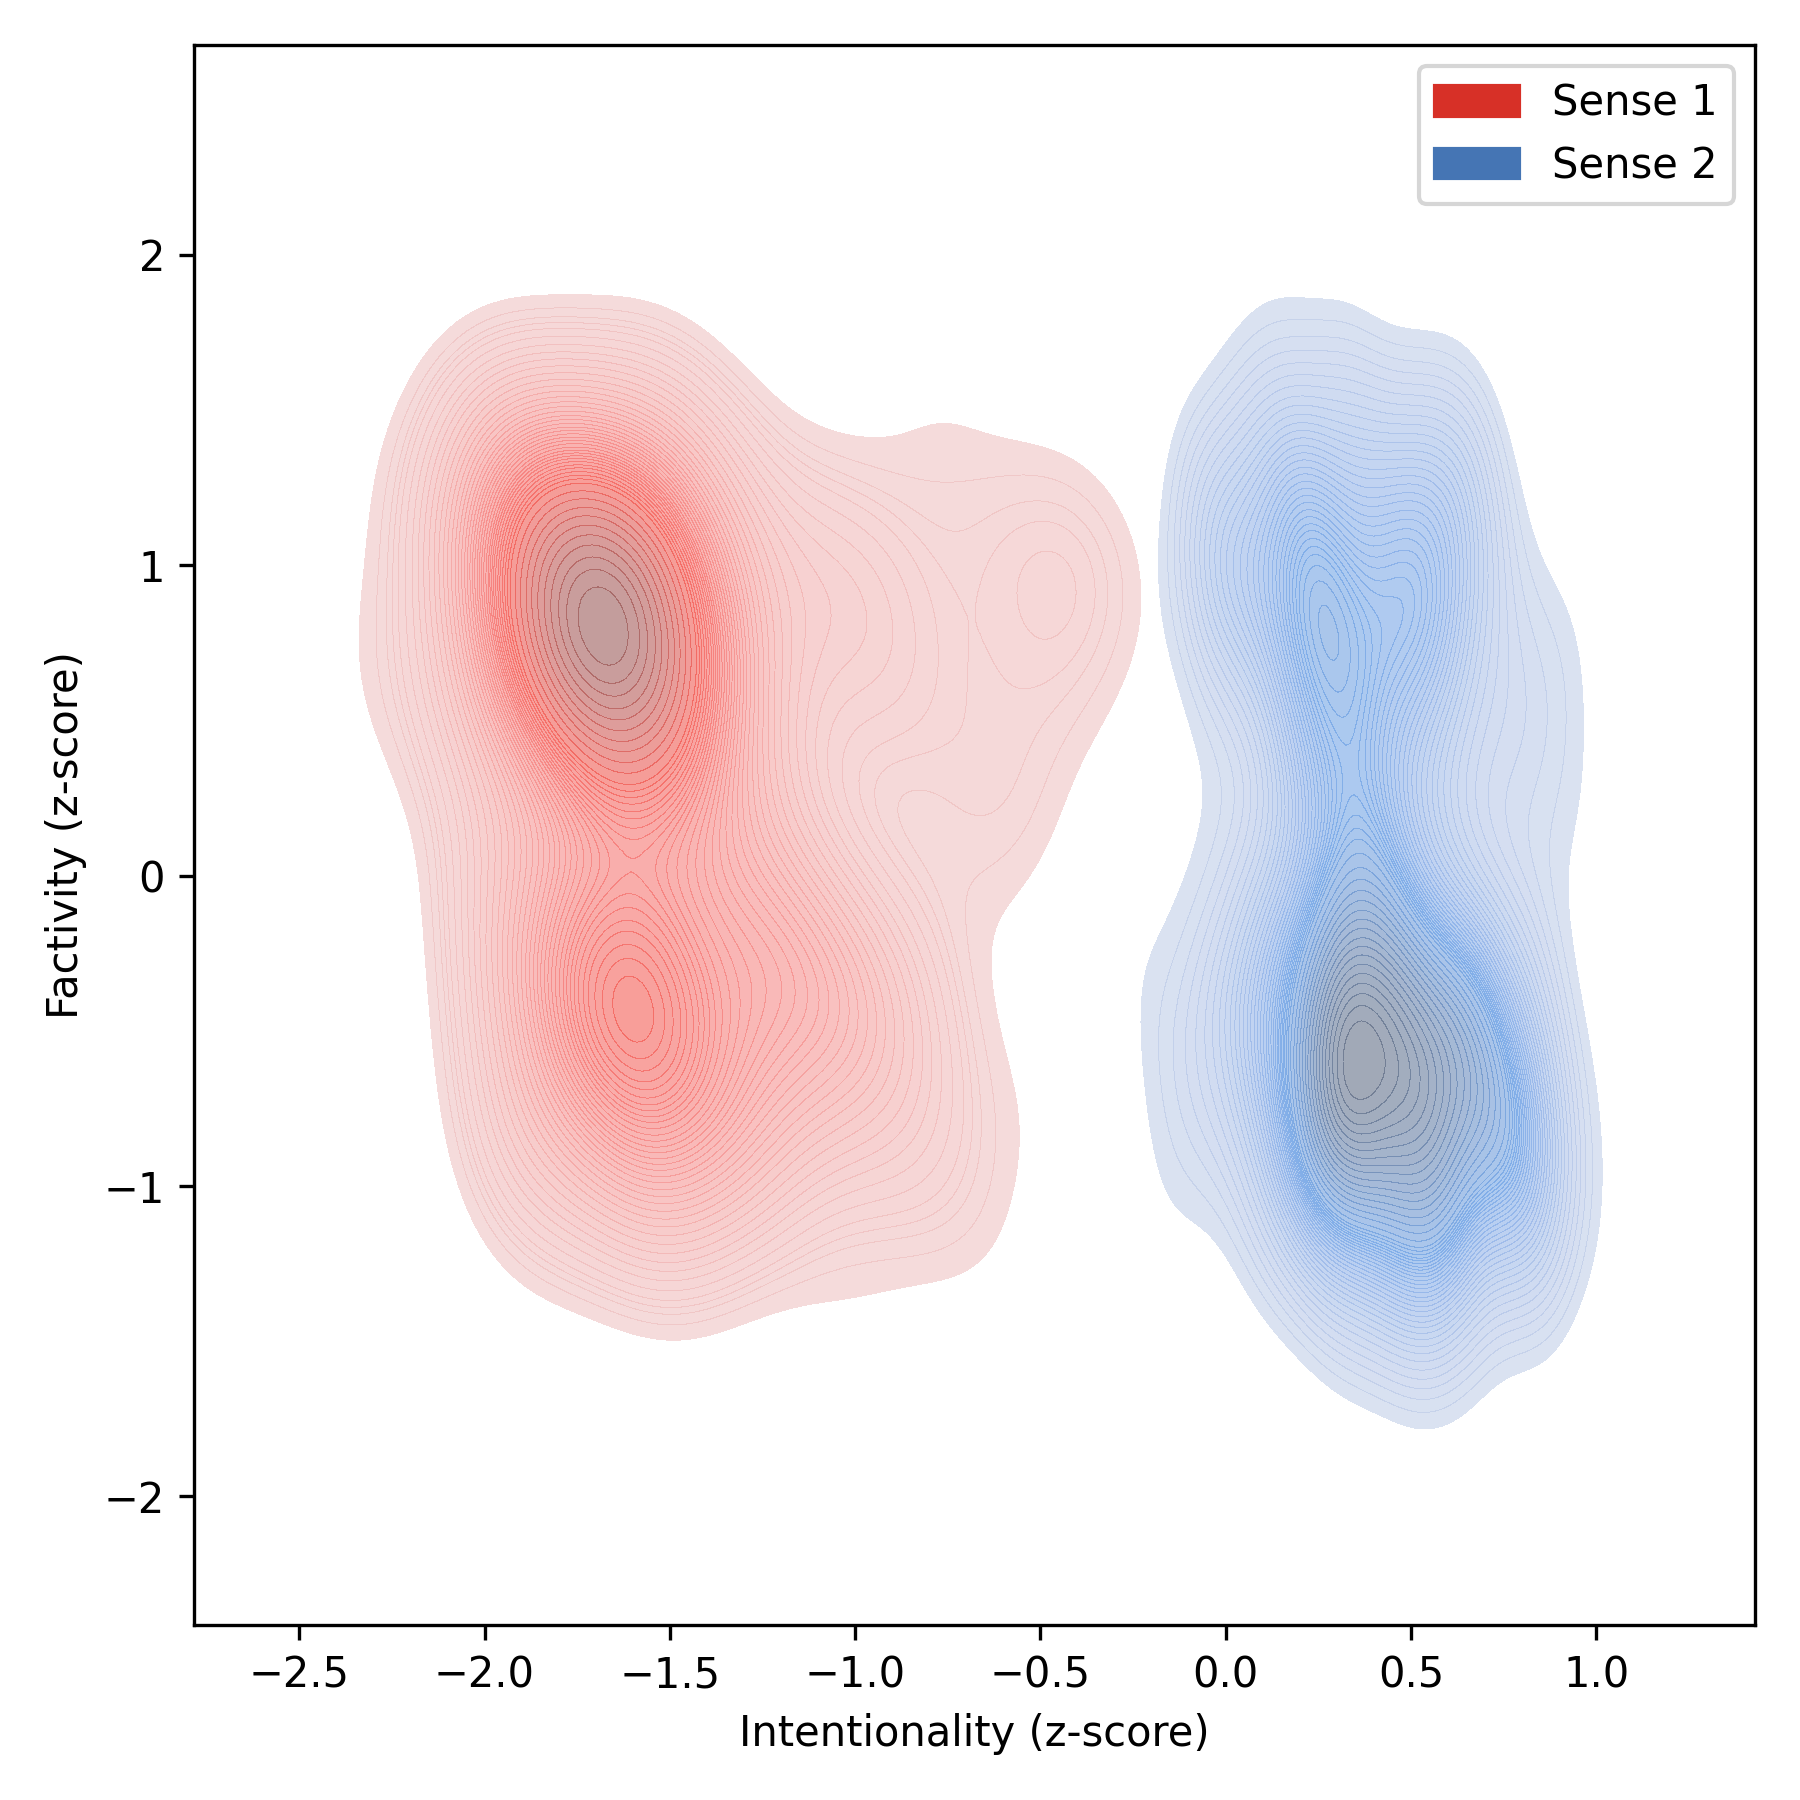
\includegraphics[width=\textwidth]{../../output/plots/embedding_projection_intentionality_z_factivity_z_2D_core.png}
    \caption{\label{fig:2D_IF}}
    \end{subfigure}
    \hfill
    \begin{subfigure}[b]{0.30\textwidth}
    \centering
    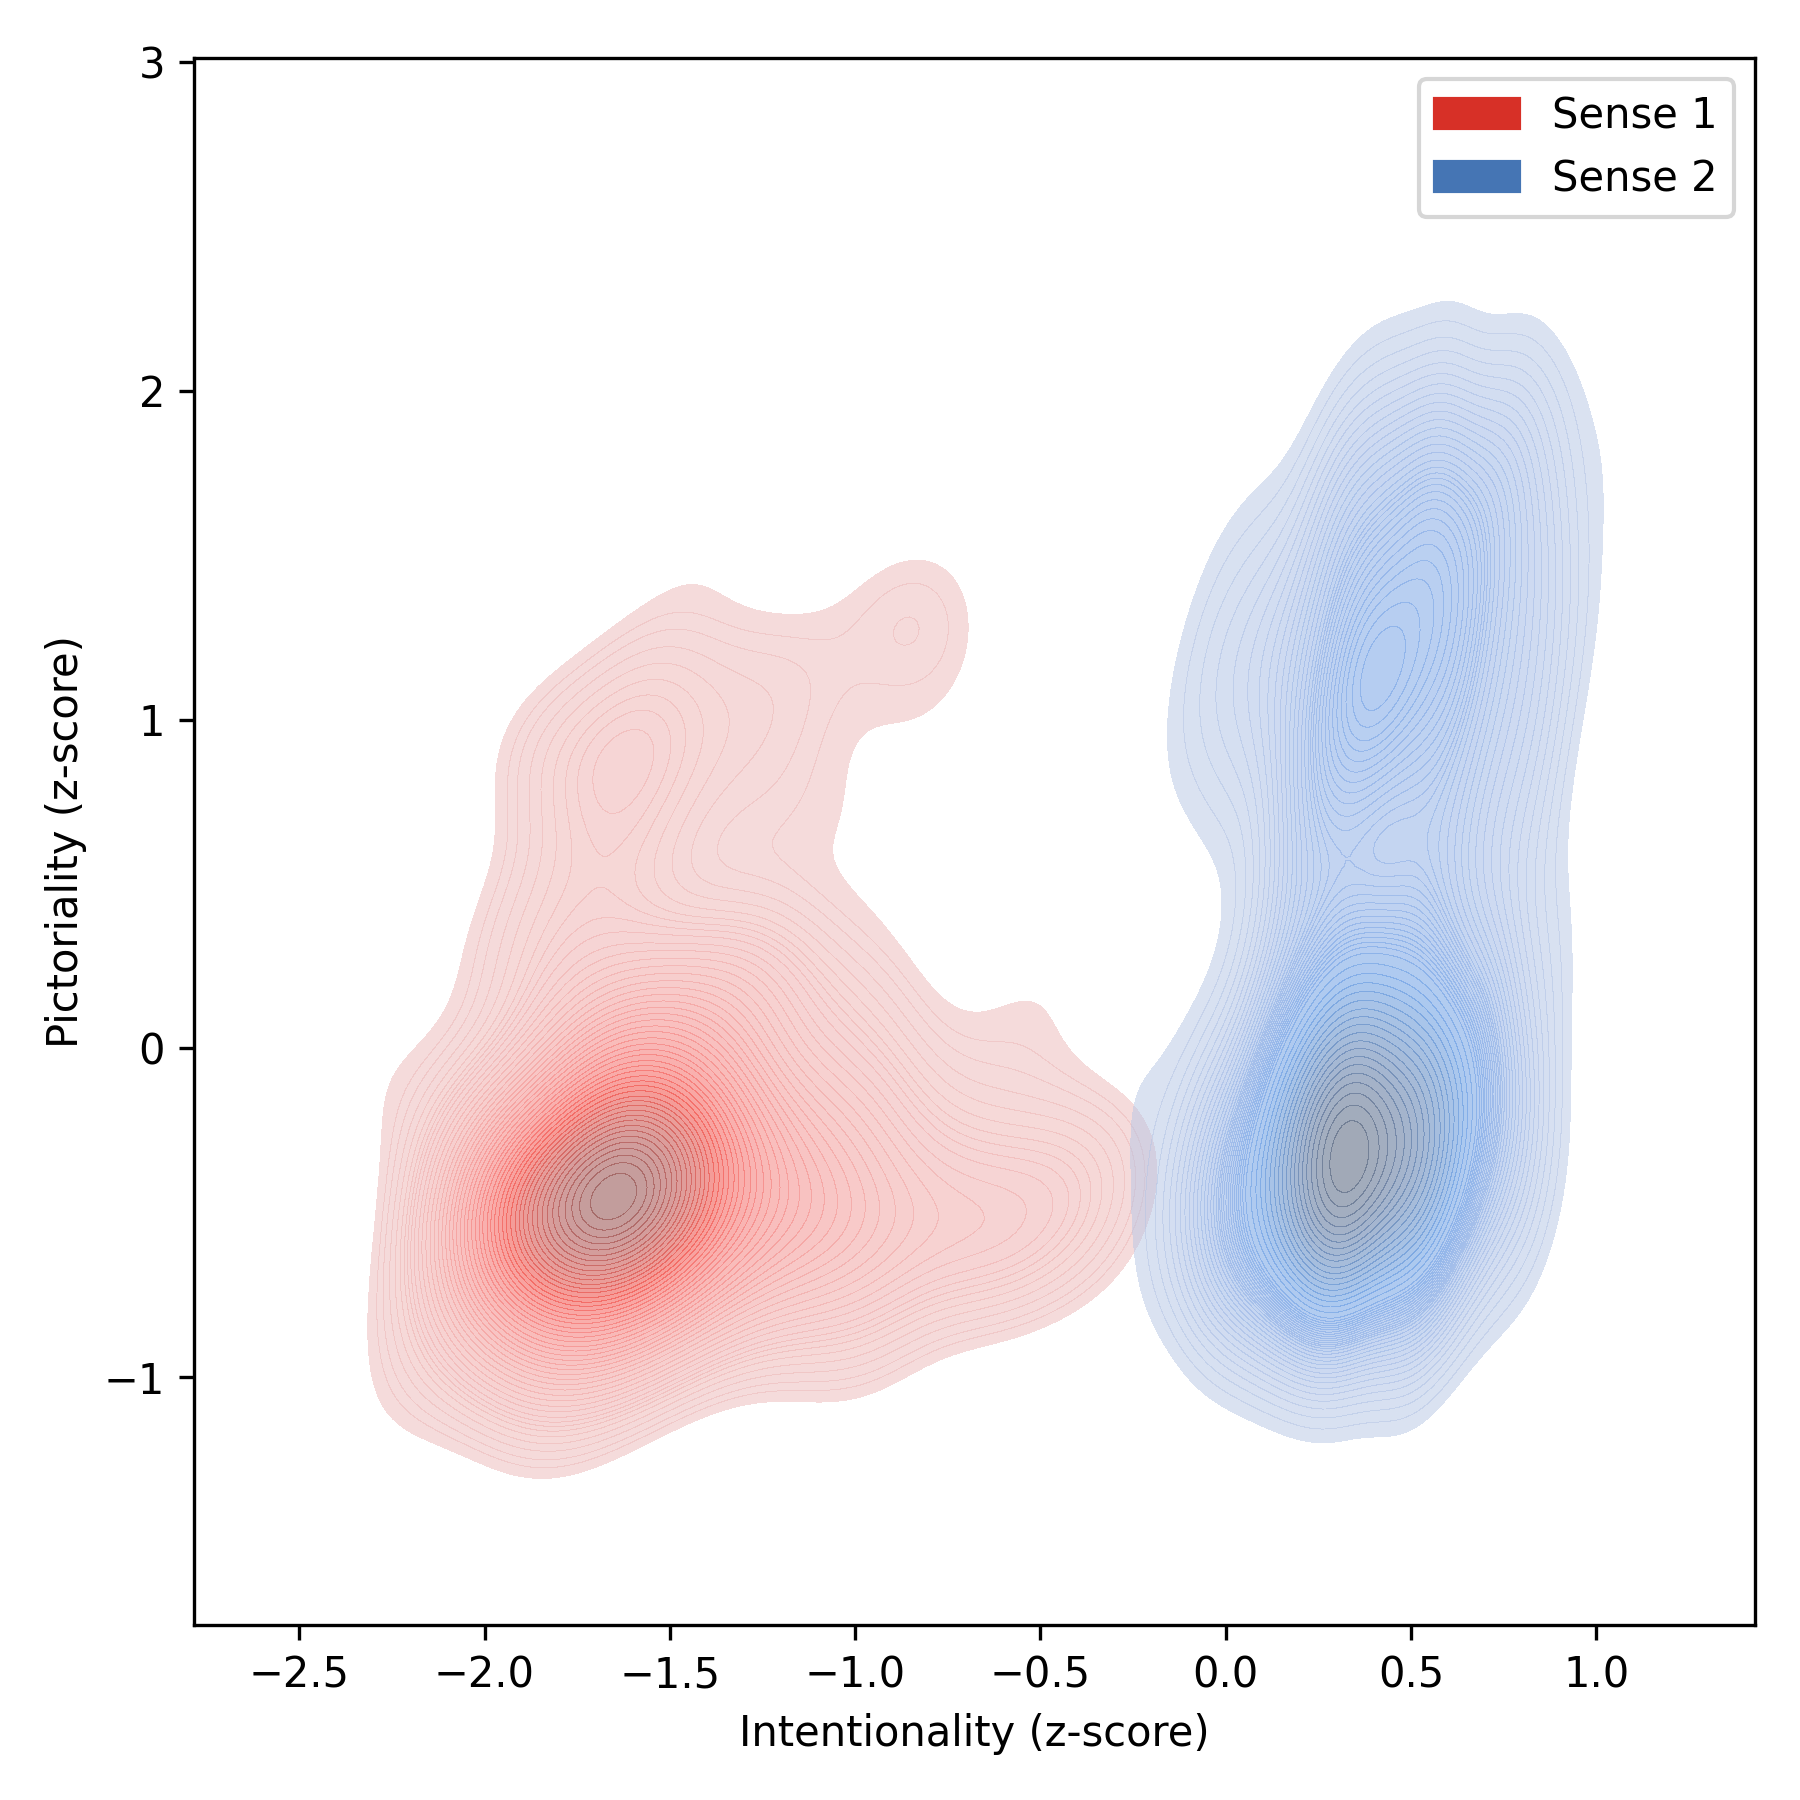
\includegraphics[width=\textwidth]{../../output/plots/embedding_projection_intentionality_z_pictoriality_z_2D_core.png}
    \caption{\label{fig:2D_IP}}
    \end{subfigure}
    \hfill
    \begin{subfigure}[b]{0.30\textwidth}
    \centering
    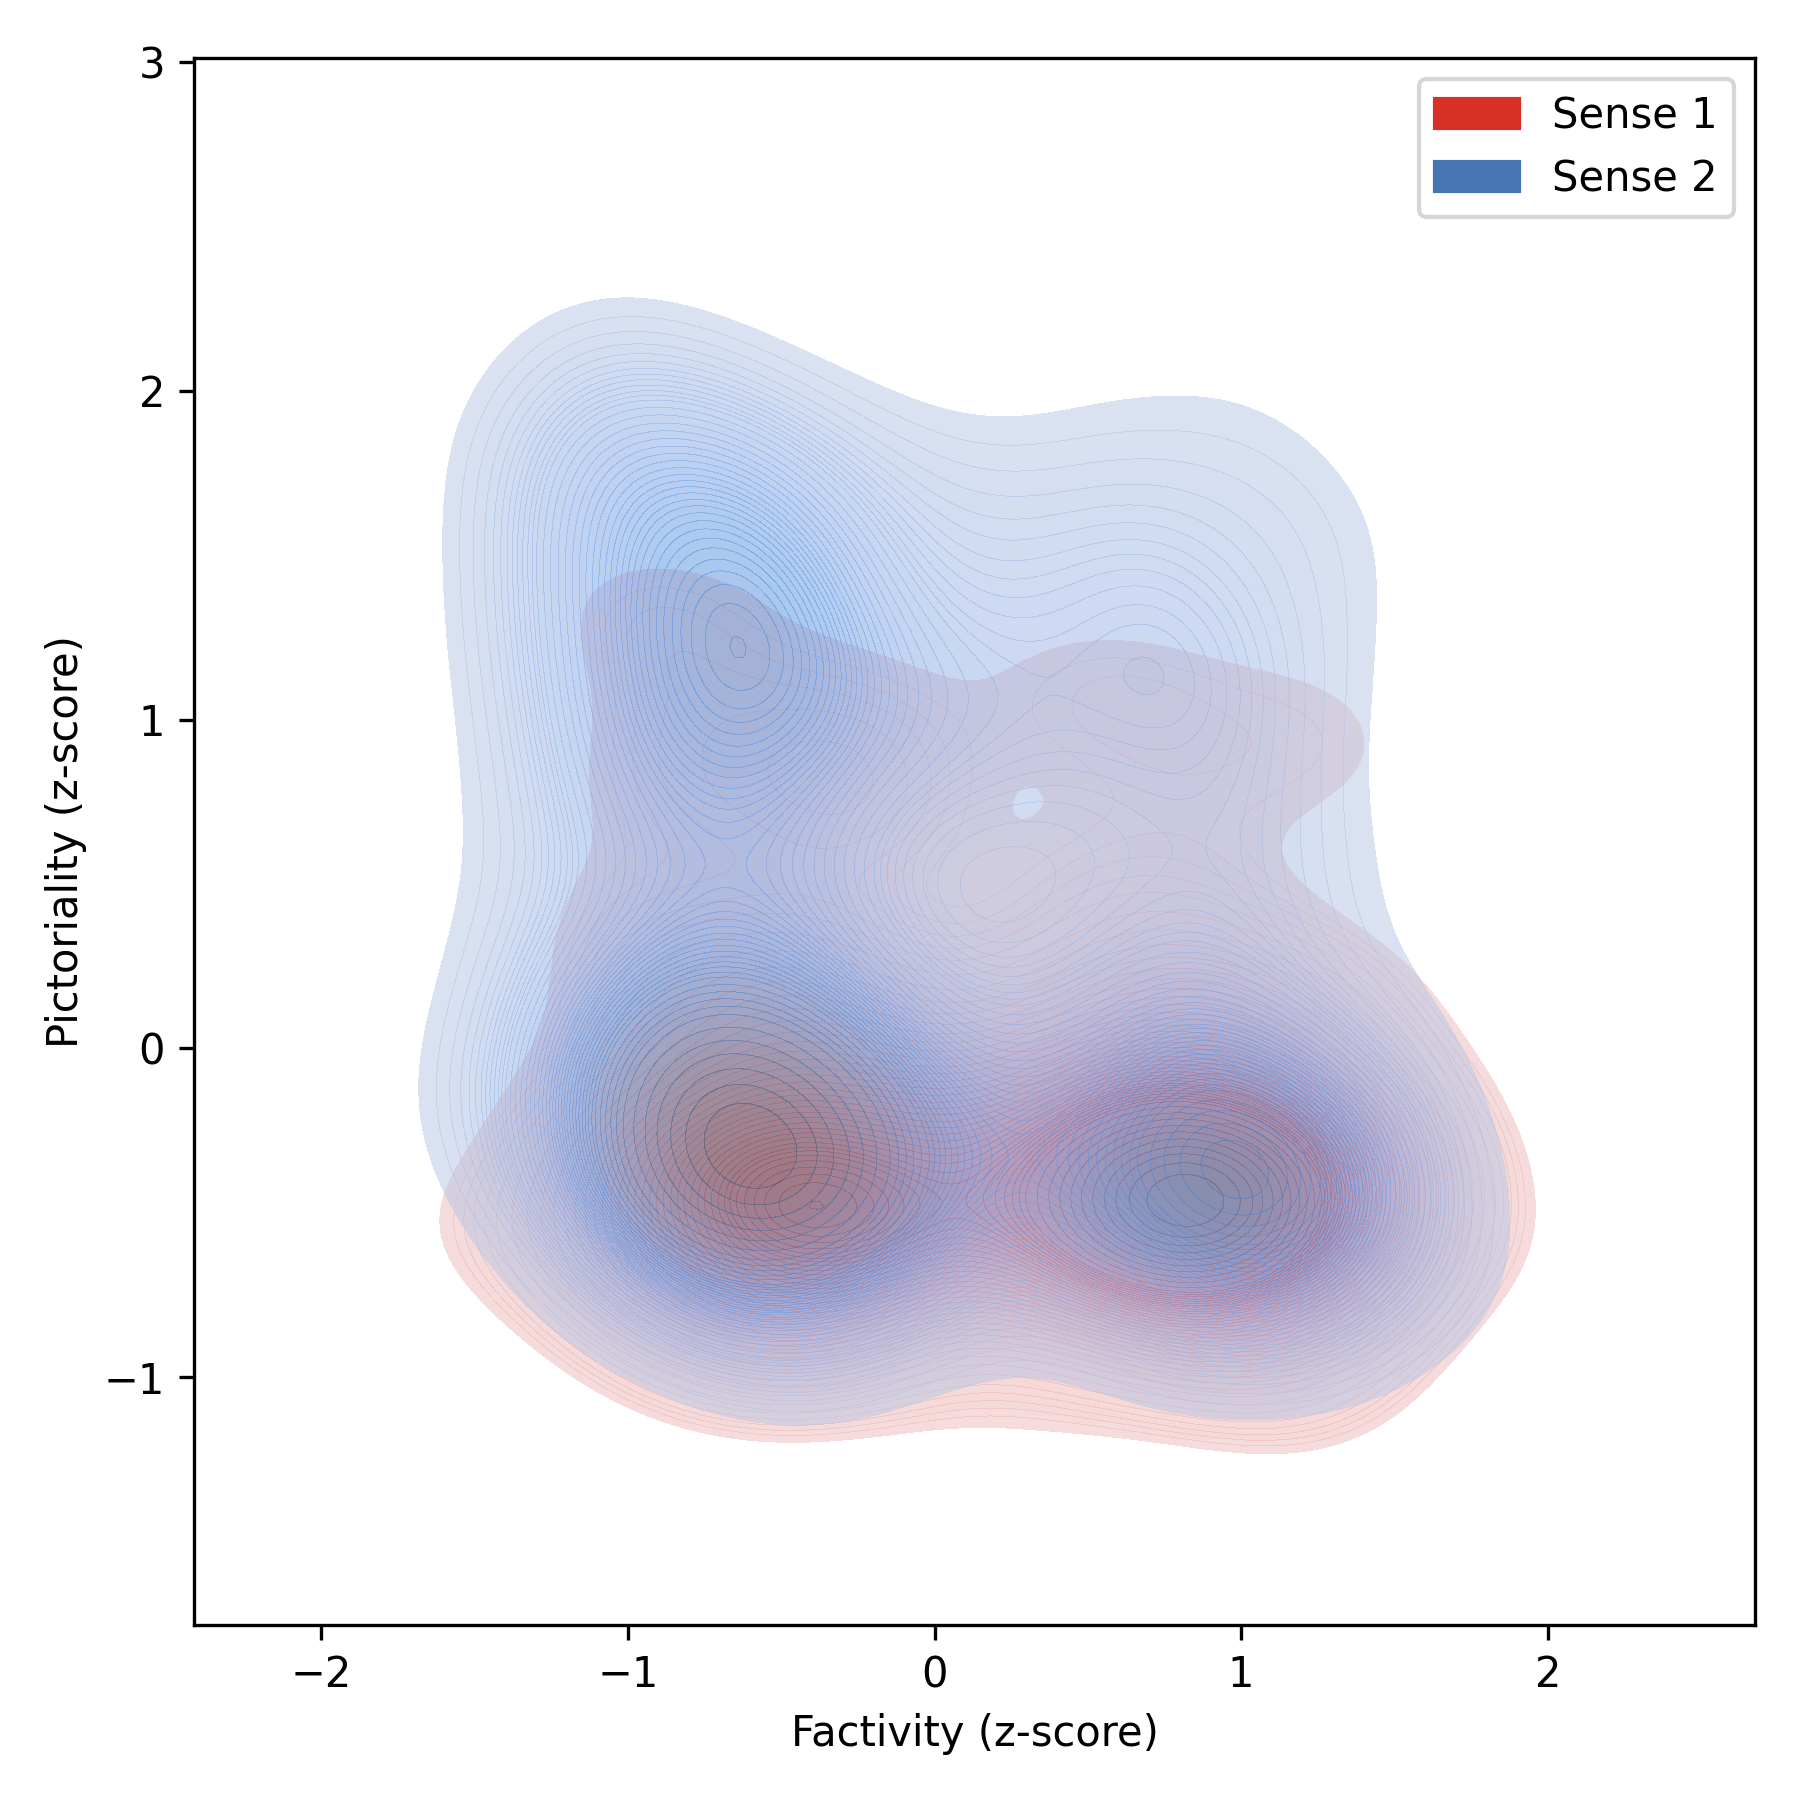
\includegraphics[width=\textwidth]{../../output/plots/embedding_projection_factivity_z_pictoriality_z_2D_core.png}
    \caption{\label{fig:2D_FP}}
    \end{subfigure}
\end{figure}

  \bibliography{hb.bib}

\end{document}
